\documentclass[11 pt]{article}
\setlength{\columnsep}{0.2in}
\usepackage[utf8]{inputenc}
\usepackage{tgtermes}
\usepackage{multicol}
\usepackage{amsmath}
\usepackage{enumitem} 
\usepackage{dsfont} 
%\usepackage{lmodern}
%\usepackage{nicefrac}
\usepackage[round]{natbib} 
\usepackage[a4paper, total={7.5in, 10in}]{geometry}
\usepackage{graphicx}
\usepackage{float}
\usepackage{booktabs} % Horizontal rules in tables
\usepackage{lettrine} % The lettrine is the first enlarged letter at the beginning of the text
%\setlist[itemize]{noitemsep} % Make itemize lists more compact
%\setlist[enumerate]{noitemsep}
\usepackage{hyperref} % For hyperlinks in the PDF
\usepackage{csquotes} %quotation
\usepackage{dirtytalk} %" " quotation in line
\def\signed #1{{\leavevmode\unskip\nobreak\hfil\penalty50\hskip2em
  \hbox{}\nobreak\hfil--- #1%
  \parfillskip=0pt \finalhyphendemerits=0 \endgraf}}
\newsavebox\mybox
\newenvironment{aquote}[1]
  {\savebox\mybox{#1}\begin{quote}}
  {\signed{\usebox\mybox}\end{quote}}
%\usepackage{titling}
\usepackage[round]{natbib} %biblio
\usepackage{epigraph}
\usepackage[usenames, dvipsnames]{color} %colours
\definecolor{mypink1}{rgb}{0.858, 0.188, 0.478}
\usepackage{cancel} %to strikeout words

%----Abstract
%\usepackage{abstract} % Allows abstract customization
%\renewcommand{\abstractnamefont}{\normalfont\bfseries} % Set the "Abstract" text to bold
%\renewcommand{\abstracttextfont}{\normalfont\small\itshape} % Set the abstract itself to small italic text

%----Title of sections
\usepackage{titlesec} % Allows customization of titles
\renewcommand\thesection{\Roman{section}} % Roman numerals for the sections
\renewcommand\thesubsection{\roman{subsection}} % roman numerals for subsections
\renewcommand\thesubsubsection{\roman{subsubsection}}
\titleformat{\section}[block]{\Large\scshape\centering}{\thesection.}{1em}{} % Change the look of the section titles
\titleformat{\subsection}[block]{\large\scshape\centering}{\thesection.\thesubsection}{1em}{} 
\titleformat{\subsubsection}[block]{\large\scshape}{\thesection\thesubsection\thesubsubsection}{1em}{} 

%\title{\vspace{-2ex}\Huge\textbf{Bayesian Variable Selection}\vspace{-2ex}}
%\author{\Large\textsc{Pietro Lesci}\thanks{Short review paper for the Bayesian statistical methods -- 20231 exam. The reference in the footnotes are inserted for the curious reader; this review is based on the four books and articles cited in the reference section. The aim of the paper at hand is to convey an overview of the variable selection problem in the normal linear regression model with focus on the Bayesian methods, however non-Bayesian methods are discussed in historical perspective.} \\
%\normalsize Università Commerciale L. Bocconi\\
%\normalsize \href{mailto:pietro.lesci@studbocconi.it}{pietro.lesci@studbocconi.it}\vspace{-2ex}}
%\date{\small 06 December 2017}
%\setlength{\droptitle}{-4 \baselineskip}


\begin{document}

%\maketitle
\newenvironment{myfont}{\fontfamily{pag}\selectfont}{\par}
\newenvironment{myfont1}{\fontfamily{put}\selectfont}{\par}
\begin{flushleft}
\begin{myfont}
\Huge\bfseries Bayesian Variable Selection
\vspace{0.3cm}
\end{myfont}
\begin{myfont1}
\Large \scshape Pietro Lesci
\end{myfont1}
\normalsize Università Commerciale L. Bocconi\\
\normalsize \href{mailto:pietro.lesci@studbocconi.it}{pietro.lesci@studbocconi.it}
\end{flushleft}

\vspace{1ex}
\rule{18cm}{.7pt}\\
\begin{citation}
 \textit{This short review paper aims, humbly, at giving a very general overview of the most important and studied methods to implement variable selection in the normal linear regression model, and at providing examples of the practical usage of these methodologies in the companion paper where the packages \texttt{BoomSpikeSlab} and \texttt{BayesVarSel} are exploited. My objective has been to be very concise and direct to core of the issues. However, a great -- huge -- part of the current literature is missing though. In particular, the NMIG method of [\cite{Ish2005}] has not been included; all the machine learning literature has not been considered and a lot of peculiar frequentist techniques have not been included/discussed deeply being the focus on the Bayesian methodologies. The references included in the footnote are for the curious reader -- basically for my-future-self -- and are not the bases on which I build this brief review. In the overwhelming literature I manage to select, with the highest care possible, the paper that I believe to be essential to approach this interesting matter; and perhaps that has been the most difficult, and at times frustrating, task. The actual algorithms to implement the techniques discussed are also included. }
\end{citation}\\
\centerline{\rule{18cm}{.7pt}}


\begin{multicols}{2}


\section{Introduction}
\setlength\epigraphwidth{.5\linewidth}
\epigraph{Variable selection is hard!}{\textsc{Ed. George}}

\lettrine[nindent=0em,lines=3]{L}inear regression has been around for a long time and is the topic of innumerable textbooks. Although it may seem somewhat dull compared to some of the more modern statistical approaches, linear regression is still a useful and widely used statistical learning method and it is the \say{experimental laboratory} for new techniques that are then applied to more complex statistical models. Why linear regression? In Gelman's words 

\begin{displayquote}
\textit{Regression: What’s it all about?
Regression plays three different important roles in applied statistics: \textit{(i)} a specification of the conditional expectation of $y$ given $X$ (used for prediction), \textit{(ii)} a generative model of the world, \textit{(iii)} a method for adjusting data to generalise from sample to population, or to perform causal inferences.} 
\end{displayquote}

Therefore, we use linear regression to assess how one quantity, $y$, varies as a function of another quantity or vector of quantities, $X$. In general, we are interested in the conditional distribution of $y$, given $X$, parameterized as $p(y|\theta, X)$.
We usually are interested in answering a few important questions too:
\begin{enumerate}
\item \textit{Is at least one of the predictors $X_1,X_2,...,X_p$ useful in predicting the response?}
\item \textit{Do all the predictors help to explain Y, or is only a subset of the predictors useful?}
\item \textit{How well does the model fit the data?}
\end{enumerate}
This review aims at presenting in a general way the different answers that has been formulated to address question 2, with special focus on the bayesian techniques. But, firstly, why go Bayesian? 
\begin{aquote}{\textsc{\cite{Joe2015}}}
\textit{For small samples, the Bayesian approach with thoughtfully well specified priors is often the only way to go because of the difficulty in obtaining well calibrated frequentist intervals...
For medium to large samples, unless there is strong prior information that one wishes to incorporate, a robust frequentist approach...is very appealing since consistency is guaranteed under relatively mild conditions. For highly complex models...a Bayesian approach is often the most convenient way to formulate the model...}
\end{aquote}
In general, suppose that we have $p$ distinct predictors. The multiple normal linear regression model takes the form
\begin{align*}
    y_i = & \; \zeta + \beta_1 x_{1,i} + ... + \beta_p x_{p,i} + \varepsilon_i, \quad \varepsilon_i \sim \mathcal{N}(0,\sigma^2)
\intertext{where $x_{j,i}$ is the $i$'th component of the $n \times 1$ vector $x_j$. In a more compact form,}
    \underset{(n \times 1)}{y} = &  \; \mathbf{1}_n\zeta + \underset{(n \times p)}{X}\underset{(p \times 1)}{\beta} + \underset{(n \times 1)}{\varepsilon}, \quad \varepsilon \sim \mathcal{N}(0,\sigma^2 I_n) 
\end{align*}
where $X = [x_1 \;  ... \; x_p]$. This is the most widely used version of the model. It follows that the distribution of $y$ given $X$ is normal with a mean that is a linear function of $X$: $E(y_i|\beta,X_i) = \beta_1x_{1,i} + ... + \beta_{p,i}$ for $i = 1,..., n$ and $X_i$ the $i$'th row of the matrix $X$.

The statistical inference problem is to estimate the parameters $\theta = (\zeta, \beta, \sigma^2)$, conditional on $X$ and $y$. In the Bayesian framework this is done as usual [\cite{Gelman2004}]: evaluating the posterior distribution of the paramenters given the data.
A full Bayesian model includes a distribution for $X$ indexed by a parameter vector $\varphi$, that is $p(X|\varphi)$ and thus involves a joint likelihood $p(y, X|\varphi, \theta)$ along with a prior distribution $p(\varphi, \theta)$. 
In the standard regression context, the distribution of $X$ is assumed to provide no information about the conditional distribution of $y$ given $X$, that is prior independence of the parameters $\theta$ and $\varphi$ is assumed. Thus from a Bayesian perspective, the defining characteristic of a \say{regression model} is that it ignores the information supplied by $X$ about $(\varphi, \theta)$. 

For simplicity, in what follows, the conditioning on $X$ will be always assumed. Therefore we are required to specify the \textit{likelihood} $p(y|\theta)$ that, given our assumption on the errors, is 
\begin{equation*}
    Y|\beta,\sigma^2 \sim \mathcal{N}_n(\mathbf{1}_n\zeta + X\beta, \sigma^2 I_n) 
\end{equation*}
and a \textit{prior} $p(\theta)$ on the parameters in order to obtain the \textit{posterior}
\begin{equation*}
    p(\theta|y) \propto \underbrace{p(y|\theta)}_{\text{the model}} \times  \;\;p(\theta)
\end{equation*}
Everything is elegantly simple, but closed-form posterior distributions for $\beta$, $\sigma^2$ and $\zeta$ are only available under restricted prior distributions; from this the need to resort to simultations to approximate the posterior (particularly used is the Gibbs sampling).

Take a few steps ahead -- actually, make a huge jump -- and let the parameters be estimated correctly whatever the methodology used. As said above, some natural questions arise: is the likelihood that we have specified the \say{best}? Is the model the most \say{efficient}? Is each of the predictor \say{useful}? Although these question might seem trivial at a first glance, in practical applications with huge datasets and possibly an infinite number of predictors available, parsimonious criteria to select the best, most efficient and most useful -- whatever the meaning that we will assign to these adjectives in what follows -- ones is necessary. Now that we have set the stage, we can go to the core of the discussion.



\section{The problem}

A very common problem in statistics is when several statistical models are proposed as plausible descriptions for certain observations $y$ and the observed data are used to resolve the \textit{model uncertainty}. This problem is normally known as model selection or model choice if the aim is to select a single “best” model, but if the model uncertainty is to be formally reflected in the inferential process, we typically use \textit{model averaging}, where inference on issues that are not model-specific (such as prediction or effects of covariates) is averaged over the set of models under consideration. A particularly important model uncertainty problem in practice is variable selection where the proposed models share a common functional form (e.g. a normal linear regression model) but differ in which explanatory variables, from a given set, are included to explain the response. There are many alternatives, both classical and modern, both frequentist and Bayesian, to implement variable selection [\cite{ISL}]:

\begin{itemize}
    \item \textit{Subset Selection}: this approach involves identifying a subset of the $p$ predictors that we believe to be related to the response
    \item  \textit{Shrinkage}: this approach involves fitting a model involving all $p$ predictors. However, the estimated coefficients are shrunken towards zero relative to the least squares estimates. This shrinkage (also known as regularization) has the effect of reducing variance. Depending on what type of shrinkage is performed, some of the coefficients may be estimated to be exactly zero. Hence, shrinkage methods can also perform variable selection
    \item \textit{Dimension Reduction}: this approach involves projecting the $p$ predictors into a $M$-dimensional subspace, where $M<p$. This is achieved by computing $M$ different linear combinations, or projections, of the variables. Then these $M$ projections are used as predictors to fit a linear regression model
\end{itemize}

We here consider only the \textit{Best Subset Selection} problem. Ideally, we would like to perform variable selection by trying out all the different models, each containing a different subset of the predictors. We can then select the best model out of all of the models that we have considered using various statistics  to judge the quality of the model based on some criteria. The number of possible models (subsets) is $2^p$ that even with a small number of predictors considered becomes intractible soon: for $p = 20$ the possible models are $2^{20} = 1,048,576$! Therefore, unless $p$ is very small, we cannot consider all $2^p$ models, and instead we need an automated and efficient approach to choose a smaller set of models to consider.


\section{Non-Bayesian approaches: long story short}

One of the first methodology was proposed by Furnival and Wilson (1974)\footnote{Furnival, G. M. and Wilson, R. W. (1974). \textit{Regressions by leaps and bounds}. Technometrics, 16(4):499–511.}, the \textit{leaps and bounds procedure}, which finds the subset $\gamma$ of each size $p_\gamma \in \{1,...,p\}$ that gives smallest residual sum of squares, yet feasible for only $p$ as large as 30 or 40. Another famous method for reduction is obtained with variants of step-wise methods that sequentially add or delete variables based on greedy considerations [e.g., Efroymson (1960)\footnote{Efroymson, M. A. (1960).  \textit{Multiple regression analysis}. Mathematical  Methods  for  Digital Computers, pp. 191–203.}]. There are three \say{modern} approaches to implement this kind of selection [\cite{ESL}]:
\begin{itemize}
    \item \textit{Forward selection}: is a greedy algorithm\footnote{It is an algorithmic paradigm that follows the problem solving heuristic of making the locally optimal choice at each stage with the hope of finding a global optimum (source: \url{https://en.wikipedia.org/wiki/Greedy_algorithm}).}, that starts with a null model that includes the intercept only and then sequentially adds into the model the predictor that most improves the fit: fits $p$ simple linear regressions and add to the null model the variable that results in the lowest $RSS$. This approach is continued until some stopping rule is satisfied. Forward selection can always be used, but since it is a greedy approach, it might include variables at first that later become redundant; mixed selection remedy this.
    
    \item \textit{Backward selection}: starts with the full model, and sequentially deletes the predictor that has the least impact on the fit. The candidate for dropping is the variable with the smallest Z-score (or higher p-value). This procedure continues until a stopping rule is reached. Backward selection can only be used when $n>p$.
    
    \item \textit{Mixed selection}: it is a combination of forward and backward selection. It starts with no variables in the model and, as with forward selection, it adds the variable that provides the best fit. It continues to add variables one-by-one. If at any point the p-value for one of the variables in the model rises above a certain threshold, it removes that variable from the model. It continues to perform these forward and backward steps until all variables in the model have a sufficiently low p-value and all variables outside the model would have a large p-value if added to the model
\end{itemize}
these methods are the standard frequentist workhorses [\cite{CSI}] for selection/reduction. Once attention is reduced to a manageable set of models, criteria are needed for selecting a subset model. The earliest developments of such selection criteria in the linear model context were based on attempts to minimise the mean squared error (MSE) of prediction. Different criteria correspond to different assumptions about which predictor values to use, and whether they are fixed or random.

For linear models many of the popular selection criteria [\cite{George2000}] are special cases of a penalised sum of squares criterion, providing a unified framework for comparisons. Assuming $\sigma^2$ known for simplicity, this general criterion selects the subset model that minimizes
\begin{align}
    RSS_\gamma/\sigma^2 + F p_\gamma
\end{align}
where $F$ is a preset \say{dimensionality penalty}, that is it measures how much to penalize $RSS_\gamma/\sigma^2 = 1 - R^2$, that is the variance not explained by the model considered, with respect to the dimension of the model $p_\gamma$. 

Perhaps the most familiar of those criteria is the \textit{Mallows} $C_p = (RSS_\gamma/\hat{\sigma}^2_{full} + 2 p_\gamma - n)$
where $\hat{\sigma}^2_{full}$ is the usual unbiased estimate of $\sigma^2$ of the full model. Two of the other most popular criteria, alternative and based on two different assumptions, are the \textit{Akaike information criterion} (AIC) and the \textit{Bayesian information criterion} (BIC). Denote by $\hat{l}_\gamma$ the maximum log-likelihood of the $\gamma$'th model, AIC selects the model that maximizes $(\hat{l}_\gamma - p_\gamma$) whereas BIC selects the model that maximizes $\left(\hat{l}_\gamma - (log\,n) \; p_\gamma/2 \right)$. Akaike (1973)\footnote{Akaike, H. (1973). \textit{Information Theory and an Extension of the Maximum Likelihood Principle}, 2nd International Symposium on Information Theory, eds. B. N. Petrov and F. Csaki, Budapest: Akademia Kiado, pp. 267-281.} motivated AIC from an information theoretic standpoint as the minimization of the Kullback-Leibler distance between the distributions of $y$ under the $\gamma$'th model and under the true model. In contrast, Schwarz (1978)\footnote{Schwarz, G. (1978). \textit{Estimating the Dimension of a Model}, The Annals of Statistics, 6, 461-464.} motivated BIC from a Bayesian standpoint, by showing that it was asymptotically equivalent (as $n \to \infty$) to selection based on Bayes factors. AIC and $C_p$ corresponds to $F = 2$, while BIC is obtained by setting $F = log\, n$. By imposing a smaller penalty, AIC and $C_p$ select larger models than BIC (unless $n$ is very small). The risk inflation criterion (RIC) proposed by Foster and George (1994)\footnote{Foster, D. P., and George, E. I. (1994). \textit{The Risk Inflation Criterion for Multiple Regression}. The Annals of Statistics, 22, 1947-1975.} puts $F = 2 log\;p$ motivating this choice as yielding the smallest possible maximum inflation in predictive risk due to selection (as $p \to\infty$). It is worth mentioning that one of the drawbacks of using a fixed choice of $F$, is that models of a particular size are favoured: small $F$ favours large models, and large $F$ favours small models. Adaptive choices of $F$ can mitigate this problem.

This is only a little selection of frequentist methodologies. From now on, we will approach the problem more formally and we will turn completely Bayesian (finally!).



%--------------------------------------------------------------------

\section{The Bayesian variable selection: \\ ex pluribus unum}


In the Bayesian framework, variable selection is a multiple testing problem where each hypothesis proposes a possible subset of $p$ potential explanatory variables initially considered. Notice that there are $2^p$ hypotheses, plus the simplest one stating that none of the variables should be used. Traditionally it has been presented with convenient specific notation that uses a $p$ dimensional binary vector $\gamma = (\gamma_1,...,\gamma_p)$ to identify models. The problem is thus transformed to the form of parameter estimation: rather than searching for the single optimal model, a Bayesian will attempt to estimate the posterior probability of all models within the considered class of models (or in practice, of all models with non-negligible probability). In many cases, this question is asked in variable-specific form: the task is to estimate the marginal posterior probability that a variable should be in the model. In testing problems, several competing hypotheses, that here are interchangeably labelled $H_i$ or $M_i$, about a phenomenon of interest are proposed. The role of statistics is to provide summaries about the evidence in favour (or against) the hypotheses once the data, $y$, have been observed. 

Therefore, the pieces we need to proceed with the analysis are the usual ones of hypothesis testing:
\begin{align*}
&\text{\textit{Hypothesis prior}} && p(H_i) \qquad i=1,...,I\\
&\text{\textit{Parameters priors}} && p(\theta|H_i) = p_i(\theta)\\ 
&\text{\textit{Likelihood}} && p(y|H_i) = \int_{\Theta_i} p(x|\theta) p_i(\theta) d\theta
\end{align*}
with $p(y|\theta_i)$ such that $\theta_i \in \Theta_i \subseteq {\rm I\!R}^k$. Assuming that one of the hypothesis, including the null, is indeed true $\sum_{i=0}^I p(H_i|y) = 1$, selection is then based on the posterior model probabilities $p(H_i|y)$, that are obtained by the Bayes' rule
\begin{align*}
    p(H_i|y) = \frac{p(y|H_i)p(H_i)}{\sum_{j=0}^I p(y|H_j) p(H_j)} = \frac{B_{i0}\pi_{i0}}{1 + \sum_{j=1}^I B_{j0} \pi_{j0}}
\end{align*}
where the last equality is obtained multiplying and dividing by $p(H_0|y)$; $B_{j0} = p(y|H_j)/p(y|H_0)$ is the Bayes factor and $\pi_{j0} = p(H_j)/p(H_0)$ are the prior odds. 
It is very useful to notice that every pair of hypotheses, even the non-nested ones, can be tested making direct reference to the null model -- which is always nested in the others, as we will soon assert. 

Intuitively, this complete specification can be understood as a three stage \textit{hierarchical model} for generating the data $y$: 
\begin{enumerate}
    \item The model $M_i$ is generated from\\ \centerline{$p(\mathcal{M}) = p(M_0,...,M_I)$}
    \item The parameter vector $\theta_i$ is generated from $p(\theta_i|M_i)$
    \item The data $y$ is generated from $p(y| \theta_i, M_i)$
\end{enumerate}
In terms of the three stage hierarchical formulation, the model selection problem becomes that of finding the model in $\mathcal{M}$ that actually generated the data, namely the model that was generated from $p(\mathcal{M})$\footnote{It is an explicit probability mass function.} in the first step.
The models' posterior distributions $p(M_0|y), ..., p(M_I|y)$ are the fundamental object of
interest for model selection. By treating $p(M_i| y)$ as a measure of the \say{truth} of model $M_i$, a natural and simple strategy for model selection can be stated:
\begin{displayquote}
\centering
\textit{Criterion: choose the $M_i$ with highest posterior probability}\footnote{Alternatively, one might prefer to report a set of high posterior models along with their probabilities to convey the model uncertainty, as it is done in the companion paper.}
\end{displayquote}

In order to set the stage for the actual implementation and analysis, consider a response variable $y$, size $n$ and a set of $p$ potential explanatory variables. The standard linear regression, as stated in the previous section, models the outcome as a linear function of the explanatory variables with a Gaussian error term. The \textit{full} model containing all the predictors can be written as 
\begin{align*}
    M_F: \; y = X_0\zeta + X \beta + \varepsilon && \varepsilon \sim \mathcal{N}_n(0, \sigma^2I_n)
\end{align*}
where the matrices $X_{0,(n\times p_0)}$, $X_{(n\times p)}$ and the vector coefficients are of conformable dimensions. Hereafter, $X_0 = \mathbf{1}_n$ is assumed to be certainly included in the true model: it is the \textit{null} model. Each $\gamma \in \{0, 1\}^p$ defines a hypothesis $H_\gamma$ stating which $\beta$’s (those with $\gamma_j = 0$) corresponding to each of the columns in $X$ are zero. Then, the model associated with $H_\gamma$ is 
\begin{align*}
    M_\gamma: \; y = \mathbf{1}_n\zeta + X_\gamma \beta_\gamma + \varepsilon && \varepsilon \sim \mathcal{N}_n(0, \sigma^2I_n)
\end{align*}
where $X_\gamma$ is the matrix with the columns in $X$ corresponding to the ones in $\gamma$ and $X_\gamma$ is an $(n \times p_\gamma)$ matrix where $p_\gamma$ is the number of 1’s in $\gamma$. Therefore, there are $2^p$ hypotheses or models plus the null model (where $\gamma = 0$ or, equivalently, $\beta = 0$) defined by
\begin{align*}
    M_0: \; y = \mathbf{1}_n\zeta + \varepsilon && \varepsilon \sim \mathcal{N}_n(0, \sigma^2I_n)
\end{align*}

Observe that we cannot test the hypotheses $H_1: \beta_1 = 0, \beta_2 \neq 0$, $H_2: \beta_1 \neq 0, \beta_2 = 0$, $H_3: \beta_1 \neq 0, \beta_2 \neq 0$ since neither $M_1$ (the model defined by $H_1$) nor $M_2$ are nested in the rest.  However, if conveniently we refer to the null model, every comparison is possible
\begin{align*}
    \frac{p(M_i)}{p(M_j)} = \frac{p(M_i)}{p(M_0)}\frac{p(M_0)}{p(M_j)} = \frac{B_{i0}}{B_{j0}}\frac{\pi_{i0}}{\pi_{j0}}
\end{align*}

 There exists at least two general ways, not strictly alternative, to frame the above structure in practice: as in \cite{George1993}, specifying a hierarchical normal mixture model or as in \cite{Kuo1998} specifying an \say{extended} normal linear model introducing the binary vector in the regression equation, thus eliminating the need for the definition of a prior on the model. In this review, in order to compare different methods, the former approach is considered, being more general and given the convenient hierarchical structure that is a useful map to follow throughout the analysis. 

%----------------------------------

\section{Models' priors}
Surely, the first choice that come to our minds is the simple and popular -- the \say{Laplace choice} [\cite{CSI}] -- (discrete) uniform distribution
\begin{equation*}
    p(\gamma|\omega) = 1/2^p
\end{equation*}
which is non-informative in the sense of favouring all models equally. Under this prior, the model posterior is proportional to the marginal likelihood $p(\gamma|y) = \frac{1}{2^p} p(y|\gamma)$ and posterior odds comparisons reduce to Bayes factor comparisons. But how do we assign a meaning to the resulting number? Jeffreys suggested a scale of evidence for interpreting Bayes factors. It is a Bayesian version of Fisher’s interpretive scale for the outcome of a hypothetical test, with coverage value (one minus the significance level) 0.95 famously constituting \say{significant} evidence against the null hypothesis.

%----------table in multicols--------------
\makeatletter
\newenvironment{tablehere}
  {\def\@captype{table}}
  {}

\newenvironment{figurehere}
  {\def\@captype{figure}}
  {}
\makeatother
%-------------------------------------------
\medskip
\begin{tablehere}
\centering
\sffamily
\resizebox{\linewidth}{!}{
\begin{tabular}{cc||ccc}
\toprule
 \multicolumn{2}{c}{\bfseries Jeffreys} &  \multicolumn{3}{c}{\bfseries Fisher}\\ \hline
Bayes Factor & Evidence for $M_i$ & Coverage & p-value  & Evidence for $M_i$\\ \hline
$< 1$ & negative &  .80 & .20 &  null\\
1-3 & barely worthwhile & .90 & .10 &borderline\\
3-20 & positive & .95 & .05 & moderate \\
 20-50& strong & .975 & .025 & substantial  \\
$>150 $ & very strong & .99 & .01 & strong \\
 &  & .995 & .005  & very strong  \\
 &  & .999 & .001  &  overwhelming\\ \bottomrule
\end{tabular}}
\end{tablehere}
\medskip



However, this prior puts most of its weight near models of size $p_\gamma = p/2$ because there are more of them. In fact, a particularity of variable selection is that it is affected by multiplicity issues: the more inferences are made, the more likely erroneous inferences are to occur  [\cite{Bayarri2012}]. This is because, and specially for moderate to large $p$, the possibility of a model showing spurious evidence is high just because many hypotheses are considered simultaneously. As concluded in [Scott and Berger (2006)] multiplicity must be controlled with the prior probabilities $p(H_\gamma)$ and the constant prior does not control for multiplicity.

Therefore alternative priors have been suggested [\cite{Practical2001}] for the specification of the prior inclusion probability $p(\gamma_j= 1)$ of the effect $\beta_j$. They are particular cases of the very flexible prior specified hierarchically as
\begin{align*}
   \underbrace{p(M_\gamma|\omega)}_{\equiv p(\gamma|\omega)} =  \prod_{j=1}^p \omega^{\gamma_j}(1-\omega)^{1-\gamma_j} =  \omega^{p_\gamma}(1-\omega)^{p-p_\gamma} 
\end{align*}
in which case the hyperparameter $\omega \in (0,1)$ is the the prior expected proportion of $x_j$'s in the model. Each $x_j$ enters the model independently of the other coefficients, with probability $p(\gamma_j = 1|\omega) = \omega$.
Note that the indicator variables $\gamma_j$'s are independent conditional on the prior inclusion probability $\omega$, but dependent marginally. This is eventually not justified in practical applications and could be relaxed by using an individual inclusion probability $\omega_j$ for each regression effect $\beta_j$.
Under this prior [\cite{George1993}], each $x_j$ enters the model independently of the other coefficients, with probability $p(\gamma_j = 1|\omega_j) = 1 - p(\gamma_j = 0|\omega_j) = \omega_j$. Smaller $w_j$ can be used to downweight $x_j$ which are costly or of less interest. Among the most popular default choices for $\omega$ as well as $\omega_j$ are
\begin{itemize}
    \item Fixed: $\omega = 1/2$, which assigns equal prior probability to each model resulting in the \say{Laplace choice} mentioned above
    \item Random: $\omega \sim Unif(0, 1)$, $\omega\sim Be(a,b)$, or $\omega_j \sim Be(a_j,b_j)$ with an individual-specific inclusion probability 
\end{itemize}

%---------------------------

\section{Parameters' priors}
For convenience\footnote{Integration over $X$ is always assumed.}, we can use the following notation, that explicate the dependence on the parameters of each model, to rewrite the models 
\begin{align*}
M_0: p_0(y|\alpha) \qquad M_\gamma: p_\gamma(y| \alpha, \beta_\gamma) \qquad \qquad \gamma \in \{0,1\}^p
\end{align*}
that is
\begin{align*}
M_0: \mathcal{N}_n\left(\mathbf{1}_n \zeta, \sigma^2I_n\right) \quad M_\gamma: \mathcal{N}_n \left(\mathbf{1}_n \zeta + X_\gamma\beta_\gamma, \sigma^2I_n \right)
\end{align*}
Note that, if the covariance matrix is of the form $\sigma^2 D$ with $D$ known, simply transform $y$ so that the covariance matrix is proportional to the identity; note that this does not alter the meaning of the $\beta_j$’s and hence the meaning of the models. Furthermore, setting $\alpha = (\zeta,\sigma)$\footnote{It is worth mentioning that in our analysis $\sigma^2$ and $\zeta$ are \say{nuisance} parameters: \say{Suppose there’s someone you want to get to know better, but you have to talk to all her friends too. They’re like the nuisance parameters.} -- Andrew Gelman.} puts this in the general framework: $\alpha$ and $\beta_\gamma$ are unknown model parameters, the latter having dimension $p_\gamma$.  Under the null model, the prior is $p_0(\alpha)$; under model $M_\gamma$, and without loss of generality, we express the model selection prior as
\begin{align*}
    p_\gamma(\alpha,\beta_\gamma) = p_\gamma(\beta_\gamma|\alpha) p_0(\alpha)
\end{align*}
Notice that $\alpha$ occurs in all of the models, so that it is referred to as the \textit{common} parameter; the $\beta_\gamma$ are called model specific parameters. The goal is to find appropriate priors both for $p_\gamma(\alpha, \beta_\gamma)$ and $p_0(\alpha)$

A key feature of Bayesian model selection, when the models have differing dimensions and non-common parameters, is that results are typically highly sensitive to the choice of priors for the non-common parameters. Prior specifications are usually difficult to impose in practical settings (which is why standard hypothesis testing is so popular) and, \say{unfortunately}, the effectiveness of the Bayesian approach rests firmly on the specification of the parameter priors. The contributions regarding this aspect have roots in Jeffreys who first proposed using proper priors centered at zero and with flat tails (Cauchy). [Zellner and Siow (1980)] extended this idea to regression problems. [Bayarri and Garcia-Donato (2007)], used such priors to test general hypotheses in linear models (regression or ANOVA). [\cite{Bayarri2012}], introduce a deep methodological change: they propose and formalise the idea of specifying (and characterizing) priors based on sensible criteria like invariance, predictive matching and consistency.

Here we consider three of the most important proposals: \textit{objective} priors, \textit{spike and slab} priors \textit{à la} \cite{George1993} and \textit{spike and slab} priors \textit{à la} \cite{Ish2005}.

\subsection{Objective priors}
If one would think to resort to improper prior for an objective analysis, she will be deluded since improper priors cannot typically be used for non-common parameters, such as $\beta$ since they do not cancel out in the Bayes factor, ruling out the use of the main tools developed in objective Bayesian estimation theory. Because of the difficulty in assessing subjective priors for numerous models, there have been many efforts (over more than 30 years) to develop “conventional” or \say{objective} priors for model selection [\cite{Bayarri2012}]. They are labelled \textit{objective model selection priors} where the word \say{objective} simply indicate that they are not subjective priors and are chosen conventionally based on the models being considered. 
[\cite{Bayarri2012}] have built the so-called \say{robust} priors that satisfy certain criteria essential for model selection priors. This has been a major innovation in this sense, therefore it is sensible to report at least the criteria that they used, skipping the details of the actual derivation of the prior. 

They group the criteria into four classes: basic, consistency criteria, predictive matching criteria and invariance criteria.
\begin{itemize}[label={}]
    \item Criterion 1 (Basic): \textit{Each conditional prior $p_\gamma(\beta_\gamma|\alpha)$ must be proper (integrating to one) and cannot be arbitrarily vague in the sense of almost all of its mass being outside any believable compact set}.
    \item Criterion 2a (Model selection consistency): \textit{If data $y$ have been generated by $M_\gamma$ , then the posterior probability of $M_\gamma$ should converge to 1 as the sample size $n\to\infty$}.
    \item Criterion 2b (Information consistency): \textit{For any model $M_\gamma$, if $\{y_m, m = 1, 2,... \}$ is a sequence of data vectors of fixed size such that, as $m\to\infty$,} 
    \begin{align*}
        \Lambda_{\gamma0}=\frac{\sup_{\alpha,\beta_\gamma} p_\gamma(y_m|\alpha,\beta_\gamma) }{\sup_\alpha p_0(y_m|\alpha)} \to \infty
    \end{align*}
    \textit{then} $B_{\gamma0}(y_m)\to \infty$
    \item Criterion 2c (Intrinsic prior consistency): \textit{Let $p_\gamma(\beta_\gamma|\alpha,n)$ denote the prior for the model specific parameters of model $M_\gamma$ with sample size $n$. Then, as $n\to\infty$ and under suitable conditions on the evolution of the model with $n$, $p_\gamma(\beta_\gamma|\alpha,n)$ should converge to a proper prior $p_\gamma(\beta_\gamma|\alpha)$, if there is such a limiting prior, it is called an intrinsic prior (this term here is used generically)}.
    \item Criterion 3 (Predictive matching): \textit{For appropriately defined \say{minimal sample size} in comparing $M_\gamma$ with $M_{\gamma'}$ , one should have model selection priors that are predictive matching. Optimal (though not always obtainable) is exact predictive matching}\footnote{Definition: \textit{The model/prior pairs $\{M_\gamma,\pi_\gamma\}$ and $\{M_{\gamma'},\pi_{\gamma'}\}$ are} predictive matching \textit{at sample size $n^\star$ if the predictive distributions $p_\gamma(y^\star|y)$ and $p_{\gamma'}(y^\star|y)$ are close in terms of some distance measure for data of that sample size. The model/prior pairs $\{M_\gamma,\pi_\gamma\}$ and $\{M_{\gamma'},\pi_{\gamma'}\}$ are} exact predictive matching \textit{at sample size $n^\star$ if $p_\gamma(y^\star|y) = p_{\gamma'}(y^\star|y)$ for all $y^\star$ of sample size $n^\star$.}}.
    \item Criterion 4a (Measurement invariance): \textit{The units ofmeasurement used forthe observations or model parameters should not affect Bayesian answers}.
    \item Criterion 4b (Group invariance): \textit{If all models are invariant under a group of transformations $G_0$, then the conditional distributions, $p_\gamma(\beta_\gamma|\alpha)$, should be chosen in such a way that the conditional marginal distributions $$p_\gamma(y|\alpha) = \int p_\gamma(y|\beta_\gamma,\alpha)p_\gamma(\beta_\gamma|\alpha)d\beta_\gamma$$ are also invariant under $G_0$.}
\end{itemize}
The \textit{robust} prior that will result from applying the criteria can be specified, under model $M_\gamma$, hierarchically as
\begin{align*}
    p_\gamma^R(\zeta, \beta_\gamma, \sigma) =& \; p(\zeta,\sigma)p_\gamma^R(\beta_\gamma|\zeta,\sigma)\\
    =& \; \sigma^{-1} \int_0^\infty \mathcal{N}_{p_\gamma}\left(0, g\Sigma_\gamma\right) p_\gamma^R(g)dg
\end{align*}
where \centerline{$\Sigma_\gamma = \text{cov}(\hat{\beta}_\gamma)=\sigma^2\left(V_\gamma'V_\gamma\right)^{-1}$}\\
with \centerline{$V_\gamma = (I_n - \mathbf{1}_n(\mathbf{1}_n'\mathbf{1}_n)^{-1}\mathbf{1}_n)X_\gamma$}
that is, the linear effect of the constant is eliminated: $X_\gamma$ is centred to have mean 0. And
\begin{align*}
     p_\gamma^R(g) = a\left[\rho_\gamma(b+n)\right]^2\left(g+b\right)^{-a+1} \mathds{1}_{\{g>\rho_\gamma (b+n)-b\}}
\end{align*}
with $a>0$, $b>0$, $\rho_\gamma \geq \frac{b}{b+n}$. This conditions ensure that $p_\gamma^R(g)$ is a proper density and that $g$ is positive. The particular choices of the hyperparamenters are variegate

\bigskip

\begin{tablehere}
\sffamily\small
\resizebox{0.7\linewidth}{!}{
\centering
\begin{tabular}{@{}ll@{}}
\toprule
\textit{Proposal} & \textit{Name (-prior)} \\ \midrule
Constant $g$ &  \\ \midrule
 $g=n$ & Unit Information    \\[\medskipamount]
 $g = p^2$&  Risk inflation criterion   \\[\medskipamount]
 $g=\max\{n,p^2\}$& Benchmark   \\[\medskipamount]
 $g = log(n)$ & Hannan-Quinn   \\[\medskipamount]
 $g_\gamma = \hat{g}_\gamma$& Local Empirical Bayes  \\[\medskipamount] \midrule
 \textbf{Random}&   \\\midrule
 $g\sim in-ga(1/2, n/2)$& Cauchy prior  \\[\medskipamount]
 $g|a \sim p(g) \propto (1+g)^{-a/2}$& hyper-g   \\[\medskipamount]
 $g|a \sim p(g) \propto (1+g/n)^{-a/2}$& hyper-g/n  \\[\medskipamount]
  $g|a \sim p(g) \propto (1+g)^{-3/2}$ & Robust    \\ 
 \footnotesize where $g>\frac{1+n}{p_\gamma + 1}-1$ & \\ \bottomrule
\end{tabular}}\\
\centering
\footnotesize\textbf{Source}: \cite{Garcia2017}
\caption{Proposals for the hyperparameter $g$.}
\end{tablehere}

\medskip

It is useful to note that $p_\gamma^R(\beta_\gamma|\zeta,\sigma)$ behaves in the tails as a multivariate Student distribution. Finally notice that for the null model the prior assumed is  $p_0(\zeta, \sigma) \; = \; \sigma^{-1}$


\subsection{Spike and slab priors}

\begin{figurehere}
\centering
\caption{Spike and slab prior distribution: an example}
    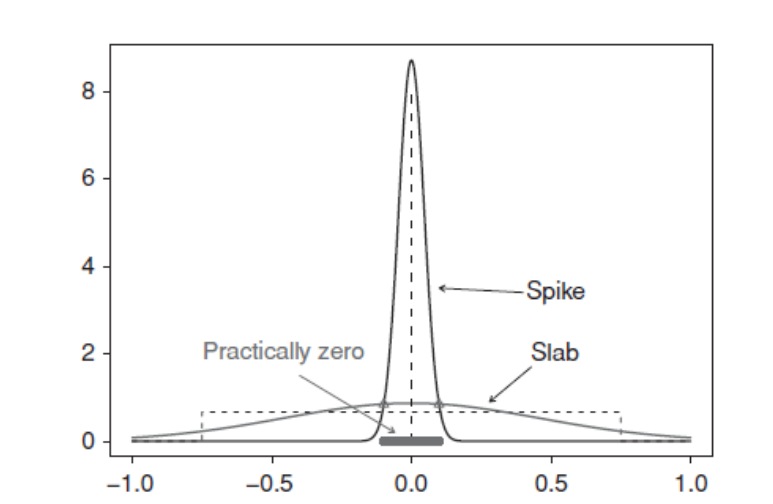
\includegraphics[width=\linewidth, keepaspectratio]{spike.PNG}
\end{figurehere}

The expression \textit{spike and slab}, has been originally coined by [Mitchell and Beauchamp (1988)]. They assume that the regression coefficients are mutually independent with a two-point mixture distribution made up of a uniform flat distribution (the slab) and a degenerate distribution at zero (the spike). In [George and McCulloch (1993)] a different prior is used. This involves a scale (variance) mixture of two normal distributions. In particular, the use of a normal prior is instrumental in facilitating efficient Gibbs sampling of the posterior. This made spike and slab variable selection computationally attractive and heavily popularised the method. 

[Ishwaran and Rao (2005)] pointed out that such normal-scale mixture priors constitute a wide class of models termed \say{spike and slab models}. They extended them to the class of \say{rescaled} spike and slab models. Rescaling was shown to induce a nonvanishing penalization effect, and when used in tandem with a continuous bimodal prior, confers useful model selection properties for the posterior mean of the regression coefficients [Ishwaran and Rao (2005)].

Mixture priors with spike and slab components have been used extensively for variable selection [\cite{Spike2011}]. The spike component, which concentrates its mass at values close to zero, allows shrinkage of small effects to zero, whereas the slab component has its mass spread over a wide range of plausible values for the regression coefficients. To specify spike and slab priors we recycle the $\gamma_j$ defined above, to be an indicator variable supported at two points $1$ and $0$. It could still be seen as a model identifier that indexes each possible subset by the vector $\gamma = (\gamma_1,..., \gamma_p)$ that is a list of zeros and ones according to whether $\beta_j$ is small or large, respectively. As above, $p_\gamma \equiv \gamma'1$  denotes the size of the $\gamma$'th subset.

The prior structure is symmetric to the one observed above: $p(\alpha, \beta) = p(\beta|\alpha)p(\alpha)$, 
with the usual uninformative prior for mean and error variance $p(\alpha) = p(\zeta, \sigma) = \sigma^{-1}$, if not differently stated.

The difficult part, as seem before, is the definition of a prior for the first term for which the same hierarchical structure to assign such prior is followed:
\begin{align*}
    \beta|\gamma &\sim p(\beta|\gamma)\\
    \gamma|\omega&\sim p(\gamma|\omega)\\
    \omega &\sim p(\omega)
\end{align*}
where, apart from the first one, everything is equal to what said in the previous subsection. Variable selection with spike and slab priors is accomplished by MCMC methods that, depending on the type of the spike specified, can be different in practical implementation.

%----independent sign
\newcommand{\indep}{\rotatebox[origin=c]{90}{$\models$}}
%------ 

In general [\cite{Spike2011}] are considered priors where regression effects allocated to the \textbf{spike} component, the $\beta_j$'s, are independent of each other and independent of $\beta_\gamma$ a priori whereas elements of $\beta_\gamma$ may be dependent; that is $$(\beta_j|\gamma_j = 0) \; \indep \; (\beta_{j^\star}|\gamma_{j^\star}=0) \; \forall \;j \neq j^\star\; \text{and} \;\indep \;\beta_\gamma$$ These spike and slab priors can be written as
\begin{align*}
    p(\beta|\gamma) = p_{slab}(\beta_\gamma) \prod_{j: \gamma_j = 0}p_{spike}(\beta_j)
\end{align*}
Once the model has been set up, the variable selection is based on the posterior probability of assigning the corresponding regression effect to the slab component, i.e. the posterior inclusion probability $p(\gamma_j = 1|y)$, given $\omega$, which can be sampled by MCMC. From this, the posterior probability that a variable is \say{in} the model, namely the posterior inclusion probability, can simply be calculated as the mean value of the indicator $\gamma_j$.

Basically two different types of \textbf{spikes} have been proposed in the literature: spikes specified by an absolutely continuous distribution and spikes specified by a point mass at zero, called Dirac spikes.

\paragraph{Absolutely continuous spikes.} To specify an absolutely continuous spike, in principle any unimodal continuous distribution with mode at zero could be used. Usually absolutely continuous spikes are combined with \textbf{slabs} where the components of $\beta_\gamma$ are independent conditional on $\gamma$, that is $$(\beta_j|\gamma_j = 1) \; \indep \; (\beta_{j^\star}|\gamma_{j^\star}=1) \; \forall \;j \neq j^\star\;$$ which, equally, can be written as
\begin{align*}
    p_{slab}(\beta_\gamma) = \prod_{j:\gamma_j=1}p_{slab}(\beta_j)
\end{align*}
Therefore,
\begin{align*}
    p(\beta|\gamma) = \prod_{j:\gamma_j=1}p_{slab}(\beta_j) \;  \prod_{j: \gamma_j 0}p_{spike}(\beta_j)
\end{align*}

Generally prior spike and slab components are specified by the \textit{same} distribution family but with a variance ratio $r$ considerably smaller than 1,
\begin{align*}
    r = \frac{\text{var}_{spike}(\beta_j)}{\text{var}_{slab}(\beta_j)} \ll 1
\end{align*}
In the majority of cases spikes and slabs which can be represented as scale mixtures of normal distributions with \textit{zero} mean are used
\begin{align*}
    \beta_j|\gamma_j, \tau^2_j \sim \mathcal{N}\left(0, r(\gamma_j)\;\tau^2_j \right) && \tau^2_j|\phi \sim p(\tau^2_j|\phi)
\end{align*}
where $r(\gamma_j)= \begin{cases} 
1 \; &\text{if} \; \gamma_j = 1\\ 
r = \text{var}_{spike}(\beta_j)/\text{var}_{slab}(\beta_j) \; &\text{if} \; \gamma_j = 0\end{cases}$ and the distribution of $\tau^2_j$ may depend on a further parameter $\phi$. 

In particular, the most used normal spikes and slabs are the ones with constant $\tau^2_j = V$, called SSVS priors where
$r$ is defined differently
$$r(\gamma_j)= \begin{cases} 
1 \; &\text{if} \; \gamma_j = 0\\ 
c^2 \; &\text{if} \; \gamma_j = 1\end{cases}$$  and the normal mixtures of inverse-gamma distributions (NMIG) priors where $\tau^2_j \sim in-ga\left(\nu, Q\right)$. Note that for the NMIG prior marginally both spike and slab component are $t$-student distributions $p_{spike}(\beta_j) = t_{2\nu}(0, c_j Q/\nu)$ and $p_{slab}(\beta_j) = t_{2\nu}(0, Q/\nu)$.

\paragraph{Dirac spikes.}  In the original proposal by Mitchell and Beauchamp (1988)\footnote{Mitchell, T. and J. Beauchamp (1988). \textit{Bayesian variable selection in linear regression}. Journal of the Americal Statistical Association 83, 1023–1032.} the spike is a degenerate distribution at zero. A Dirac spike is specified as $$p_{spike}(\beta_j) = p(\beta_j|\gamma_j=0) = \Delta_0(\beta_j)$$ where $\Delta_0$ is a Dirac Delta function, therefore having zero variance, the spike and slab prior perfectly expresses the original variable selection criterion of either accepting or rejecting a variable. The formulation requires the computation of a full posterior distribution and in the absence of a convenient conjugacy relationship, the only way out is to do MCMC sampling.

Dirac spikes are combined with \textbf{slab} components of the form
\begin{align*}
    p_{slab}(\beta_\gamma) = \mathcal{N}_n(a_{\gamma,0}\;,A_{\gamma,0}\; \sigma^2)
\end{align*}
where particular assumptions on the parameters $a_{\gamma,0}$ and $A_{\gamma,0}$ are
\begin{itemize}
    \item the independence slab (i-slab), where $a_{\gamma,0} = 0$ and $A_{\gamma,0} = c I_n$
    \item the $g$-slab, where $a_{\gamma,0} = 0$ and $A_{\gamma,0} = g\;(X_\gamma'X_\gamma)^{-1}$
    \item the fractional slab (f-slab), where $a_{\gamma,0} = (X_\gamma'X_\gamma)^{-1}X_\gamma'y$ and $A_{\gamma,0} = \frac{1}{b}(X_\gamma'X_\gamma)^{-1}$
\end{itemize}
Recall that $X_\gamma$ is the design matrix consisting only of those columns of $X$ corresponding to non-zero effects, i.e. where $\gamma_j =1$. The g-slab is Zellner’s g-prior [Zellner (1986)] for such effects. The f-slab is the corresponding fractional prior [O’Hagan (1995)]. The idea of the fractional prior is to use a fraction $b$ of the likelihood to determine a prior distribution for the parameters. In this specification the f-slab is not a fraction of the whole likelihood, but only of the part containing information on the regression coefficients $\beta$. Note that in contrast to the i-slab, regression coefficients $\beta_j$ are not independent conditional on $\gamma$ for g- and f-slab where the joint distribution of all effects with
$\gamma_j=1$ is specified with a variance-covariance matrix.
However, their mean is different: the g-slab is centred at the null vector, whereas the mean of f-slab is the LS estimate of the regression effects with $\gamma_j = 1$.



\subsection{Stochastic search variable selection} 
A particular example of absolutely continuous spike and slab priors is the one implemented in the SSVS [\cite{George1997}] approach: the spike is a narrow distribution concentrated around zero. A mixture prior for $\beta_j$ is used
\begin{align}
    p(\beta_j | \gamma_j) = (1 - \gamma_j)\; \mathcal{N}(0, \tau^2_j) \;+\; \gamma_j\;\mathcal{N}(0, c^2\tau^2_j) \label{SSVS}
\end{align}
where the first density (the spike) is centred around zero and has a small variance. When $\gamma_j = 0$, $\beta_j|\gamma_j \sim \mathcal{N}(0, \tau^2_j)$ and when $\gamma_j = 1$, $\beta_j|\gamma_j \sim \mathcal{N}(0, c^2\tau^2_j)$.

The interpretation of this formulation is that: first, $\tau_j (>0)$ is set small so that if $\gamma_j = 0$, then $\beta_j$ would probably be so small that is could be estimated by zero. Second, $c (>1)$ is set large so that if $\gamma_j = 1$, then a non-zero estimate of $\beta_j$ should probably be included in the final model. 

To obtain \eqref{SSVS} as the prior for $\beta_j|\gamma_j$, a multivariate normal prior is defined
\begin{align}
    \beta|\gamma \sim \mathcal{N}_p (0, D_\gamma R D_\gamma) \label{SSVSmult}
\end{align}
where $R$ is the prior correlation matrix of $\beta$ conditionally on $\gamma$ and it is a tuning constant that calibrates the information in $p(\gamma|y)$. Its effect on the posterior covariance matrix of $\beta$ under $p(\beta|y, \sigma^2,\gamma)$ can be assessed from the following formula that stems from the conjugacy of the prior
\begin{align*}
    \left(\frac{1}{\sigma^2}X'X+D_\gamma^{-1}R^{-1}D_\gamma^{-1}\right)^{-1}
\end{align*}
Particularly interesting are the special cases $R=I_{(n \times n)}$ and $R\propto \left(X'X\right)^{-1}$ which can be considered as extremes. In the first case, the component of $\beta$ are independent under $p(\beta|\gamma)$. In the second case, the prior correlation is identical to the design correlation: a generalisation of the $g$-prior. 

$D_\gamma \equiv diag[z_1\tau_1,...,z_p\tau_p]$ with $z_j = 1$ if $\gamma_j = 0$ and $z_j = c_j$ if $\gamma_j = 1$. This matrix determines the scaling of the prior covariance matrix. Also in this multivariate context, $\tau_1,...,\tau_p$ are set small and $c_1,...,c_p$ are set large so that if $\gamma_j = 0$ in \eqref{SSVSmult}, $\beta_j$ will tend to be clustered around 0, while if $\gamma_j = 1$ they will be more dispersed. Therefore, coupled with $p(\gamma|\omega)$, the prior on $\beta$ is a finite mixture of multivariate normal priors.

The last ingredient is a prior on the residual variance $\sigma^2$ for which we define a conjugate inverse-gamma prior
\begin{align*}
    \sigma^2|\gamma \sim in-ga \left(\frac{\nu_0}{2}, \frac{\nu_0\sigma^2_0}{2}\right)
\end{align*}
In choosing the hyperparameters, one may use the interpretation that these carry information from an imaginary prior experiment where $\nu_0$ is the number of observations (prior sample size) and $[\nu_0/(\nu_0-2)]\sigma^2_0$ is the prior estimate of $\sigma^2$.

Tuning is not easy, as $p(\beta_j | \gamma_j = 0)$ needs to be very small but at the same time not too restricted around zero otherwise Gibbs sampler moves between states $\gamma_j = 0$ and $\gamma_j = 1$ are not possible in practice. 

\paragraph{Gibbs sampling.} Therefore, after having specified the hierarchical normal mixture model so that the posterior $p(\gamma|y)$ puts most weight on the more promising subsets, it is time to extract this information. Rather than calculate all $2^p$ posterior probabilities in $p(\gamma|y)$, the SSVS uses the Gibbs sampler to generate a sequence $$\gamma^{(1)},...,\gamma^{(s)}$$ which usually converges rapidly in distribution to $\gamma \sim p(\gamma|y)$. With high probability, in many cases, this sequence will contain exactly the information relevant to variable selection [\cite{George1997}]. This in because those $\gamma$ with highest probability will also appear most frequently and hence will be easiest to identify. Those $\gamma$ that appear infrequently or not at all are simply not of interest. 

SSVS implements Gibbs sampler to generate an auxiliary Gibbs sequence $$\beta^{(0)}, \sigma^{2(0)}, \gamma^{(0)},..., \beta^{(i)}, \sigma^{2(i)}, \gamma^{(i)},...$$ that is an ergodic Markov Chain in which the sequence of $\gamma$ is embedded. $\beta^{(0)}$ and $\sigma^{2(0)}$ are initialized to be the least square estimates of the full regression model, while $\gamma^{(0)} \equiv (1,1,...,1)$. The successive values of $\beta^{(i)}, \sigma^{2(i)}, \gamma^{(i)}$ are obtained by successively simulating values according to the following iterated sampling scheme:

\begin{enumerate}[noitemsep]
    \item sample $\beta^{(i)}$ from \begin{align*}\beta^{(i)}&\sim p(\beta^{(i)}|y, \sigma^{2(i-1)}, \gamma^{(i-1)}) \\ &= \mathcal{N}_p\Big(A_{\gamma^{(i-1)}}(\sigma^{2(i-1)})^{-1})X'X \hat{\beta}_{\text{LS}}, A_{\gamma^{(i-1)}}\Big)\end{align*}
    where 
    \begin{align*}
A_{\gamma^{(i-1)}}=&\Big((\sigma^{2(i-1)})^{-1}X'X + D_{\gamma^{(i-1)}}^{-1}R^{-1}D_{\gamma^{(i-1)}}^{-1}\Big)^{-1}\\
D_{\gamma}^{-1}=&\;diag\left[(z_1\tau_1)^{-1},...,(z_p\tau_p)^{-1}\right]
    \end{align*}
    \item sample variance $\sigma^{2(i)}$ from the updated distribution of $\sigma^2$
\begin{align*}
\sigma^{2(i)} \sim  p\left(\sigma^{(i)}|y,\beta^{(i)}, \gamma^{(i-1)}\right)\end{align*}
$$in-ga\left(\frac{n+\nu_{\gamma^{(i-1)}}}{2}, \frac{|y-X\beta^{(i)}|^2 + \nu_{\gamma^{(i-1)}}\sigma^2_{0,\gamma^{(i-1)}}}{2}\right)$$
    \item the vector $\gamma^{(i)}$ is obtained componentwise by sampling consecutively (and in random order, preferably) from the conditional distribution \begin{align*}
        \gamma_j^{(i)} &\sim p\left(\gamma_j^{(i)}|y,\beta^{(i)}, \sigma^{(i)}, \gamma^{(i)}_{-j}\right) \\ & = p\left(\gamma_j^{(i)}|\beta^{(i)}, \sigma^{(i)}, \gamma^{(i)}_{-j}\right)
    \end{align*}
    where $\gamma^{(i)}_{-j}$ indicates the vector $\gamma^{(i)}$ without the $j$-th component. Note that it does not depend on $y$ and this is the result of the hierarchical structure where $\gamma$ affects $y$ only through $\beta$. Each distribution of $\gamma_j^{(i)}$ is Bernoulli with probability $$p\left(\gamma_j^{(i)}=1|\beta^{(i)}, \sigma^{(i)}, \gamma^{(i)}_{-j}\right) = \frac{v}{v+w}$$ where 
    \begin{align*}
    v = p\left(\beta^{(i)}|\gamma^{(i)}_{-j}, \gamma^{(i)}_j = 1\right) &\times\\ p\left(\sigma^{(i)}|\gamma^{(i)}_{-j}, \gamma^{(i)}_j = 1\right) & p\left(\gamma^{(i)}_{-j}, \gamma^{(i)}_j = 1\right)\\
 w=p\left(\beta^{(i)}|\gamma^{(i)}_{-j}, \gamma^{(i)}_j = 0\right) &\times\\ p\left(\sigma^{(i)}|\gamma^{(i)}_{-j}, \gamma^{(i)}_j = 0\right) &p\left(\gamma^{(i)}_{-j}, \gamma^{(i)}_j = 0\right)
    \end{align*}
 Note that when $R = I_{(n\times n)}$ the dependence on $\gamma_{-j}^{(i)}$ vanish throughout.
\end{enumerate}
At this point the relevant information is contained in the sequence $\gamma^{(1)},...,\gamma^{(s)}$. In particular, after the sequence has reached approximate stationarity, the values of $\gamma$ corresponding to the most promising subsets of $x_1,...,x_p$ will appear with the highest frequency. Therefore, a simple tabulation of the high-frequency values of $\gamma$ can be used to identify the corresponding subsets. If no high-frequency values of $\gamma$ appear, the one would conclude that either $s$ (the number of samples) is too small or the data contain little information for discriminating among models.

\subsection{Indicator model selection} 
The most direct approach to variable selection is to insert the indicator $\gamma_j$ in regression model, that is
$$y_i = \zeta + \sum_{j=1}^p \gamma_j\beta_j x_j,i + \varepsilon_i$$
and set the slab $\beta_j | \gamma_j = 1$ equal to $\beta_j$, and the spike $\beta_j | \gamma_j = 0$ equal to 0. This approach has given given birth to two methods, differing in the way they treat $\beta_j | \gamma_j = 0$:

 
 \begin{figurehere}
\centering
\caption{Kuo \& Spike and slab prior}
    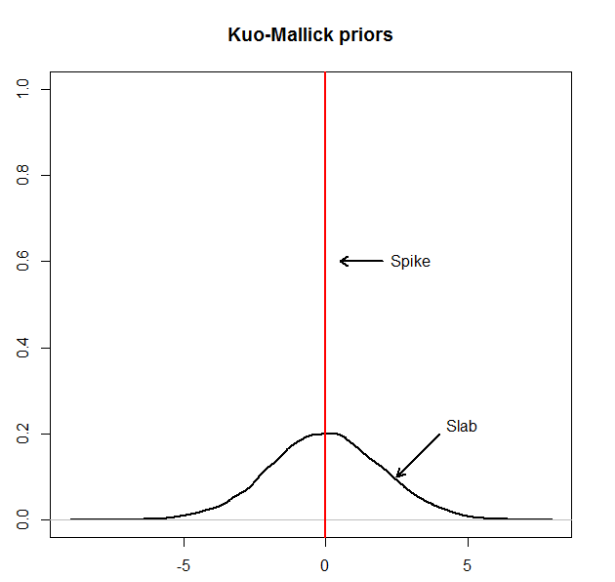
\includegraphics[width=\linewidth, keepaspectratio]{kuo.PNG}
\end{figurehere}
 
 \paragraph{Kuo \& Mallick.} The first method simply assumes that the indicators and effects are independent a priori, so $p(\gamma_j, \beta_j) = p(\gamma_j)p(\beta_j)$, and independent priors are placed on each $\gamma_j$ and $\beta_j$. The prior on each regression
coefficient is a mixture of a point mass and an absolutely continuous component. The MCMC algorithm to fit the model does not require any tuning, but when $\gamma_j = 0$, the updated value of $\beta_j$ is sampled from the full conditional distribution, which is its prior distribution -- in the paper by [\cite{Kuo1998}] there is included the analytic derivation which mathematically shows that when $\gamma_j = 0$ the data do not provide any information on the $\beta_j$. Mixing will be poor if this is too vague, so the sampler will only rarely flip from $\gamma_j = 0$ to $\gamma_j = 1$.

\paragraph{GVS.} The Gibbs Variable Selection method attempts to circumvent the problem of sampling $\beta_j$ from too vague a prior by sampling $\beta_j | (\gamma_j = 0)$ from a \say{pseudo-prior}, i.e. a prior distribution which has no effect on the posterior. The prior distributions of indicator and effect are assumed to depend on each other, that is $p(\gamma_j, \beta_j) = p(\beta_j | \gamma_j)p(\gamma_j)$ where a mixture prior is assumed for $\beta_j$: $p(\beta_j | \gamma_j) = (1-\gamma_j)\mathcal{N}(\tilde{\mu}, S)+\gamma_j\mathcal{N}(0, \tau^2)$ where constants $(\tilde{\mu}, S)$ are user-defined tuning parameters, and $\tau^2$ is a fixed prior variance of $\beta_j$. The intuitive idea is to use a prior for $\beta_j | (\gamma_j = 0)$ which is concentrated around the posterior density of $\gamma_j\beta_j$, so that when $\gamma_j = 0$, $p(\beta_j | \gamma_j = 1)$ is reasonable large, and hence there is a good probability that the chain will move to $\gamma_j = 1$. The algorithm does require tuning, i.e. $(\tilde{\mu}, S)$ need to be chosen so that good values of $\beta_j$ are proposed when $\gamma_j = 0$. The data will determine which values are good but without directly influencing the posterior, and hence tuning can be done to improve mixing without changing the model’s priors.

\section{Inference the posterior:\\general case}
For both types of spike and slab priors posterior inference is feasible using MCMC methods, where the model parameters $(\zeta, \gamma, \beta, \omega, \sigma^2)$ and additionally, under the NMIG prior, the scale parameters $\tau^2 = (\tau^2_1,...,\tau^2_p)$ are sampled from their conditional posteriors. Depending on the type of the spike component, different sampling schemes have to be used:
\begin{itemize}
    \item for an absolutely continuous spike the indicators $\gamma_j$ can be sampled conditionally on the effects $\beta_j$
    \item for a Dirac spike it is essential to draw $\gamma$ from the marginal posterior $p(\gamma|y)$ integrating over the parameters subject to selection that requires evaluation of marginal likelihoods in each MCMC iteration
\end{itemize}
In normal regression models with conjugate priors analytic integration over the regression effects is feasible and hence marginal likelihoods can be
computed rather cheaply. 

\paragraph{MCMC for absolutely continuous spikes.} For priors with an absolutely continuous spike the full conditional distribution of $(\gamma, \tau^2)$ is given as
\begin{align*}
    p(\gamma,\tau^2|\beta,\sigma^2,\omega,\zeta,y) \propto & \prod_{j=1}^p p(\beta_j|\gamma_j,\tau^2_j)p(\gamma_j|\omega)p(\tau^2_j)p(\omega) \\
    \propto & \prod_{j=1}^p p(\tau^2_j|\gamma_j,\beta_j)p(\gamma_j|\beta_j,\omega)
\end{align*}
Therefore, $\gamma$ and $\tau^2$ can be sampled together in one block and the sampling scheme involves the following steps:
\begin{enumerate}
    \item sample $\zeta$ from its posterior $\zeta|\sigma^2,y \sim \mathcal{N}(\bar{\zeta}, \sigma^2/n)$
    \item sample $\gamma$ and $\tau^2$:
        \begin{enumerate}
            \item for $j = 1, ..., p$ sample $\gamma_j$ from $$p(\gamma_j=1|\beta_j,\omega)= \frac{1}{1+\frac{1-\omega}{\omega}\frac{p_{slab(\beta_j)}}{p_{spike}(\beta_j)}} $$
            \item for normal spikes and slabs, set $\tau^2_j \equiv V$. For $t$-student spikes and slabs, where $\tau^2_j \sim in-ga(\nu,Q)$, sample $\tau^2_j$ from its conditional posterior $$\tau^2_j|\gamma_j, \beta_j \sim in-ga\left(\nu+\frac{1}{2}, Q + \frac{\beta_j^2}{2\;r(\gamma_j)} \right)$$
        \end{enumerate}
    \item sample $\omega$ from $\omega \sim Be(a + p_\gamma, b + p - p_\gamma)$
    \item sample $\beta$ from the normal posterior $\mathcal{N}(a_n,A_n)$ where $A_n^{-1} = \frac{1}{\sigma^2}(X'X)^{-1}+D^{-1}$ and $a_n = A_n X'y$ and $D$ is a diagonal matrix with entries $r(\gamma_j)\tau^2_j$, $j = 1, ..., p$
    \item sample the error variance $\sigma^2$ from the posterior $\sigma^2|y, \beta \sim in-ga(s_n, S_n)$, where
    $s_n = (n - 1)/2$ and $S_n = \frac{1}{2}(y -X\beta)'(y -X_\beta)$
\end{enumerate}

\paragraph{MCMC for a Dirac spikes.} For a Dirac spike $\gamma_j = 0$ implies $\beta_j = 0$ and viceversa. To avoid reducibility of the Markov chain, it is essential to draw $\gamma$ from the marginal posterior
\begin{align*}
    p(\gamma|y) \propto p(y|\gamma)p(\gamma) 
\end{align*}
where effects subject to selection are integrated out. Recall that $p(y|\gamma)$ denotes the marginal likelihood of the linear regression model with design matrix $X_\gamma$. For Dirac spikes combined with i-, g- or f-slab on $\beta_\gamma$ the marginal likelihood can be derived analytically
\begin{align*}
    p(y|\gamma) = \frac{1}{\sqrt{n}(2\pi)^{s_n}}\frac{|A_{\gamma,n}|^{\frac{1}{2}}}{|A_{\gamma,0}|^\frac{1}{2}}\frac{\Gamma(s_n)}{S_n^{s_n}}
\end{align*}
where $s_n = (n - 1)/2$ and $S_n = \frac{1}{2}(y'y - a_{\gamma,n}'A_{\gamma,n}^{-1}a_{\gamma,n})$. $a_{\gamma,n}$ and $A_{\gamma,n}$ are parameters of the posterior of $\beta_\gamma$:
\begin{itemize}
    \item $A_{\gamma,n}=((X_\gamma'X_\gamma) + \frac{1}{c}I_n)^{-1}$ for the i-slab
    \item $A_{\gamma,n} = \frac{g}{g+1}(X_\gamma'X_\gamma)^{-1}$ for the $g$-slab
    \item $A_{\gamma,n} = (X_\gamma'X_\gamma)^{-1}$ for the f-slab
\end{itemize}
the posterior mean is $a_{\gamma,n} = A_{\gamma,n}X_\gamma'y$ for any of the three slabs. 

With this marginalisation it is possible to sample the parameters $\gamma$, $\sigma^2$ and $\zeta$ in one block. Hence, the MCMC scheme for Dirac spikes involves the following steps
\begin{enumerate}
    \item sample $(\gamma, \sigma^2, \zeta)$ from the posterior $$p(\gamma|y)p(\sigma^2|y, \gamma)p(\zeta|y, \gamma, \sigma^2)$$
    \begin{enumerate}
        \item sample each element $\gamma_j$ of the indicator vector $\gamma$ separately from $p(\gamma_j = 1|\gamma_{-j}, y)$ given as $$p(\gamma_j = 1|\gamma_{-j}, y) = \frac{1}{1+\frac{1-\omega}{\omega}\frac{p(y|\gamma_j=0|\gamma_{-j})}{p(y|\gamma_j=1|\gamma_{-j})}}$$
        where $\gamma_{-j}$ denotes the vector $\gamma$ consisting of all elements of $\gamma$ except $\gamma_j$. Elements of $\gamma$ are updated in a random permutation order
        \item sample the error variance $\sigma^2$ from $$in-ga(s_n, S_n)$$
        \item sample the mean $\zeta$ from $N(\bar{\zeta}, \sigma^2/n)$
    \end{enumerate}
    \item sample $\omega$ from $\omega \sim Be(a + p_j, b + p - p_j)$
    \item set $\beta_j = 0$ if $\gamma_j = 0$ and sample the non-zero elements in $\beta_\gamma$ from the normal posterior $\mathcal{N}(a_{\gamma,n},A_{\gamma,n}\sigma^2)$
\end{enumerate}
For both $g$- and f-slab, the posterior variance covariance matrix $A_{\gamma,n}$ is a scalar multiple of the prior variance covariance matrix $A_{\gamma,0}$. Thus for computing the marginal likelihood, the determinant of $A_{\gamma,n}$ is not required which speeds up sampling compared to i-slabs.


\section{Other Bayesian approaches: a brief overview}


\subsection{Adaptive shrinkage} 
A different approach to inducing sparseness -- level of complexity of the model -- is not to use indicators in the model, but instead to specify a prior directly on $\beta_j$ that approximates the \say{slab and spike} shape with a prior $\beta_j | \tau^2_j \sim \mathcal{N}(0, \tau^2_j )$, and a suitable prior placed on $\tau^2_j$ to give the appropriate shape to $p(\beta_j)$. Notice that this is the usual way of stating the priors in the normal model, with the assumption of an effect-specific variance. The prior should work by shrinking values of $\beta_j$ towards zero if there is no evidence in the data for non-zero values (i.e. the likelihood is concentrated around zero). Conversely, there should be practically no shrinkage for data-supported values of covariates that are non-zero. The method is adaptive in the sense that the degree of sparseness is defined by the data, through the way it shrinks the covariates effects towards zero. The degree of sparseness of the model can be adjusted by changing the prior distribution of $\tau^2_j$ either by changing the form of the distribution or the parameters. A problem is that there is no indicator variable to show when a variable is \say{in} the model, however one can be constructed by setting a standardised threshold $c$ such that $\gamma_j = 1$ if $|\beta_j| > c$.

A scale-invariant Jeffreys’ prior can be defined on $\tau^2_j$: $p(\tau^2_j) \propto 1/\tau^2_j$ and provides one method
for adaptive shrinkage. Theoretically, the resulting posterior is not proper although a proper approximation can be made by giving finite limits to $p(\tau^2_j)$. There is no tuning parameter in the model, which is either good or bad: the slab part of the prior is then uninformative but cannot be adjusted.

An alternative is to define an exponential prior for $\tau^2_j$ with a parameter $k$. After analytical integration over the variance components, one obtains a Laplacian double exponential distribution for $p(\beta_j | k)$. The degree of sparseness is controlled by $k$ which has a data dependent scale and requires tuning. The random effect variant of the method, where $k$ is a parameter and has its own prior, is better known as the Bayesian Lasso.
 
\section{Conclusion}
In this short review paper I have tried to convey the most important and studied methods to implement variable selection in the normal linear regression model, and to provide the practical usage of these methodologies in the companion paper where the packages \texttt{BoomSpikeSlab} and \texttt{BayesVarSel} are exploited. A great -- huge -- part of the current literature is missing though. In particular, the NMIG method of [\cite{Ish2005}] has not been included; all the machine learning literature has not been considered and a lot of peculiar frequentist techniques have not been included being my focus on the Bayesian methodologies. I would like to consider the work at hand as a first sketch of an enormous picture: useful as a starting point for a future dive in this most important aspect of statistics which entails, to be understood (deeply), an holistic knowledge that cares of the highest theoretical issues (especially for the prior used, perhaps the most difficult thing I have faced) as well as of the most practical matters such as computational capabilities of PCs.
 


\bibliographystyle{apalike}
\bibliography{biblio}
\end{multicols}
\end{document}